\subsection*{Problem 5: LQR State Feedback Setpoint Tracking}
\subsubsection*{a) Design a state feedback controller to drive $\phi$ → 0 and $z$ → 0.5 m and to satisfy the aforementioned
    design requirements.}
$\bar{A}$, $\bar{B}$, and $\bar{C}$ were determined in Project 1 for the State Feedback Setpoint Tracking, therefore, their derivation will not be reiterated here.

$\bar{Q}$, $\bar{R}$, and $\bar{K}$ were designed using the following methodology. The addition of a new error state for setpoint tracking demands the $Q$ matrix be expanded to a $5\times5$ matrix. This means there is now a diagonal term that unit scales the max error using Bryson's rule. Through trial and error, the terms in this new $\bar{Q}$ were set by multiplying the existing values from Problem 3 and setting the new diagonal value to 100. This is shown in the following:

\begin{equation*}
    \begin{split}
        \bar{Q} & =
        \begin{bmatrix}
            33.06 & 0  & 0     & 0  & 0   \\
            0     & 10 & 0     & 0  & 0   \\
            0     & 0  & 26.87 & 0  & 0   \\
            0     & 0  & 0     & 10 & 0   \\
            0     & 0  & 0     & 0  & 100 \\
        \end{bmatrix}
    \end{split}
\end{equation*}

The value for $\bar{R}$ was left a 1 as in Problem 3. The controller performance was initially tested with the values of $Q$ from Problem 3 while setting the last diagonal equal to 1, but this configuration did not comfortably meet the design requirements. This is why the above changes were made. The resulting $\bar{K}$ was determined using the same methods in MATLAB from Problem 3 with $\bar{A}$ and $\bar{B}$ instead of $A$ and $B$.

\begin{equation*}
    \begin{split}
        \bar{K} & =
        \begin{bmatrix}
            -16.08 & -11.37 & 48.81 & 10.01 & -10 \\
        \end{bmatrix}
    \end{split}
\end{equation*}

The following figures depict the outputs and input of the linear system with the above controller:

\begin{figure}[!ht]
    \centering
    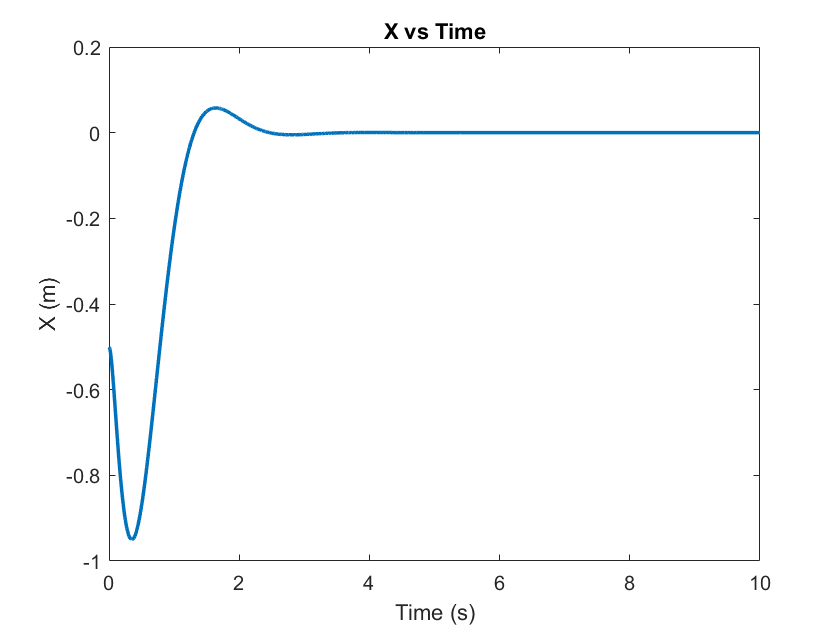
\includegraphics[width=\linewidth]{figs/sfsp_x.png}
    \caption{Linear System X Output}
    \label{}
\end{figure}

\begin{figure}[!ht]
    \centering
    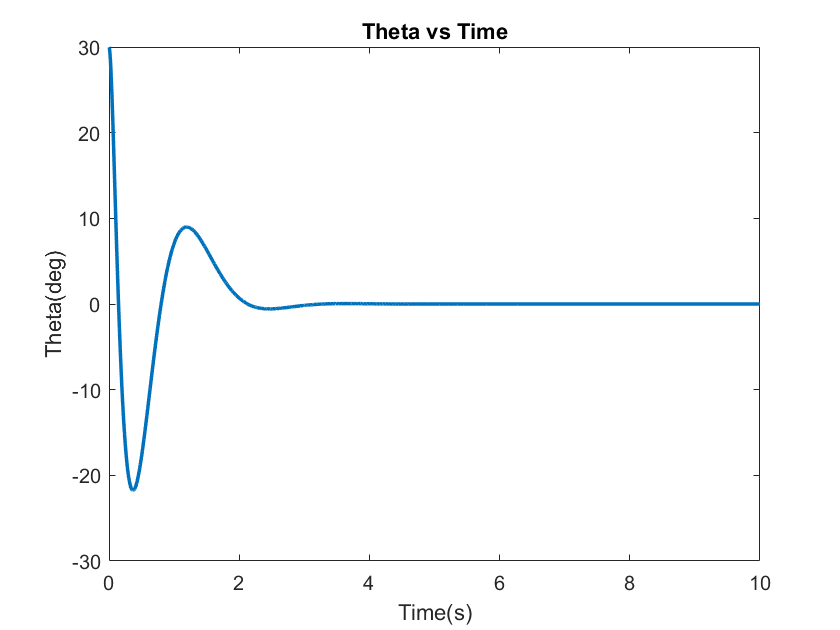
\includegraphics[width=\linewidth]{figs/sfsp_theta.png}
    \caption{Linear System $\theta$ Output}
    \label{}
\end{figure}

\begin{figure}[!ht]
    \centering
    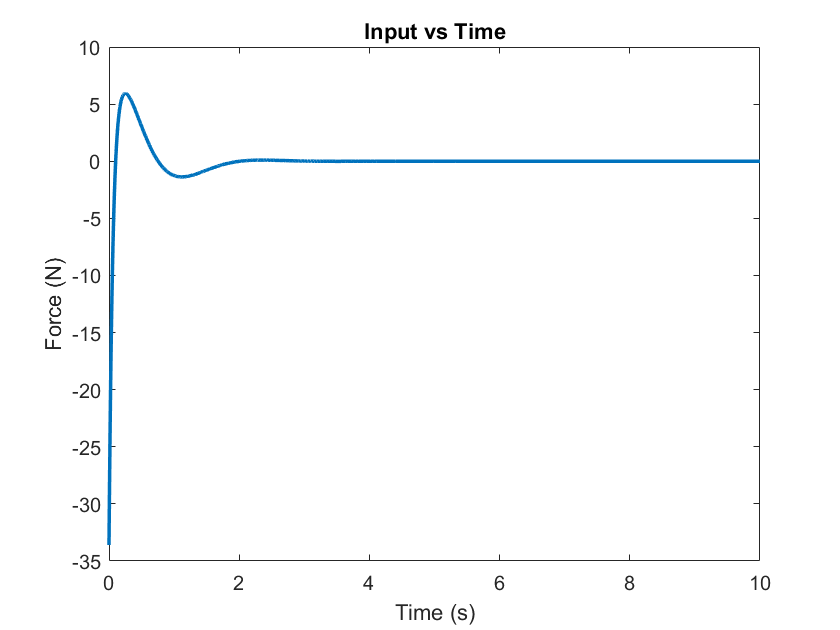
\includegraphics[width=\linewidth]{figs/sfsp_input.png}
    \caption{Linear System Input}
    \label{}
\end{figure}

\clearpage

The closed-loop eigenvalues are found from $det(sI-(A-BK))=0$. They are the following:

\begin{equation*}
    \begin{split}
        s & = -0.57\pm0.51, -5.13, -6.10
    \end{split}
\end{equation*}

\subsubsection*{b) Design the controller for the nonlinear model.}

The $\bar{Q}$, $\bar{R}$, and $\bar{K}$ used for the nonlinear system are the same as for the linear model.

The following figures depict the outputs and input of the nonlinear system with the above controller:

\begin{figure}[!ht]
    \centering
    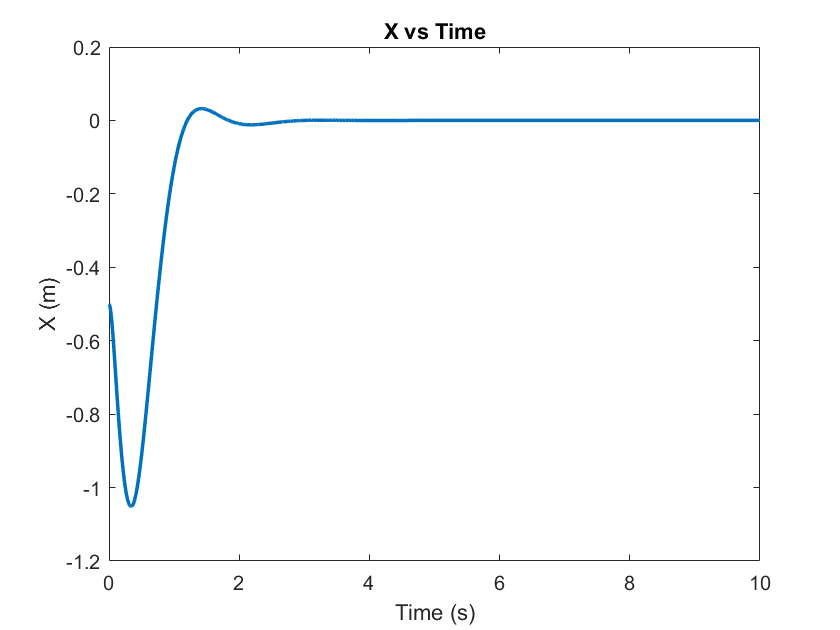
\includegraphics[width=\linewidth]{figs/sfsp_nlin_x.png}
    \caption{Nonlinear System X Output}
    \label{}
\end{figure}

\begin{figure}[!ht]
    \centering
    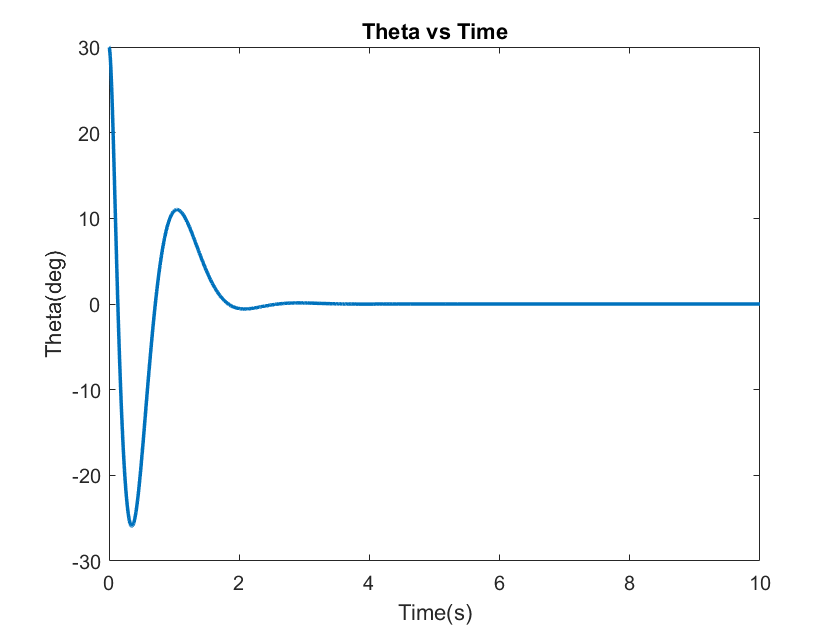
\includegraphics[width=\linewidth]{figs/sfsp_nlin_theta.png}
    \caption{Nonlinear System $\theta$ Output}
    \label{}
\end{figure}

\begin{figure}[!ht]
    \centering
    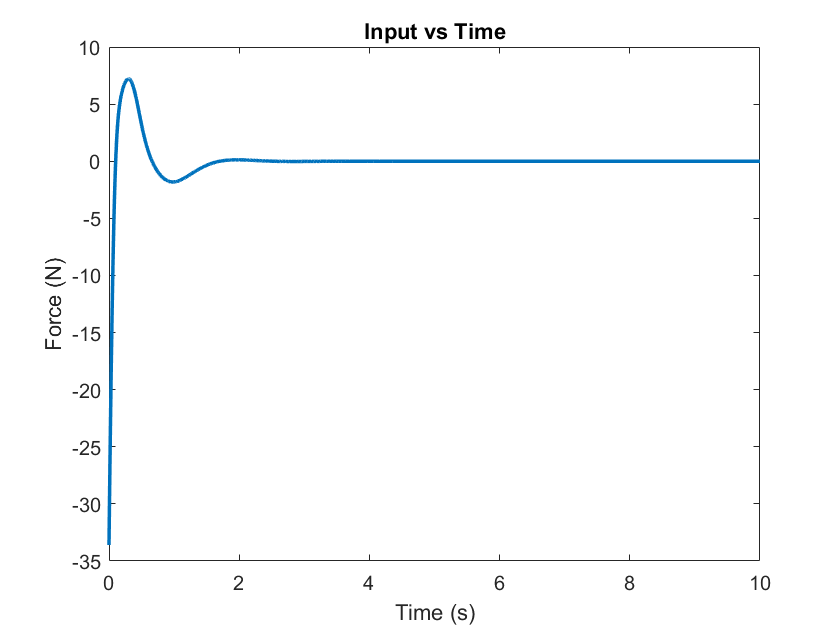
\includegraphics[width=\linewidth]{figs/sfsp_nlin_input.png}
    \caption{Nonlinear System Input}
    \label{}
\end{figure}


